\documentclass[conference]{IEEEtran}

\ifCLASSINFOpdf
\else
\fi

\hyphenation{op-tical net-works semi-conduc-tor}

\usepackage{graphicx}
\usepackage{array}
\usepackage{rotating}
\usepackage{tabularx}
\usepackage{epstopdf}
\usepackage[mathletters]{ucs}
\usepackage{mathtools}
\usepackage{amsfonts}
\usepackage{morefloats}
\usepackage{lipsum}
\usepackage{amsthm,amsmath}


\usepackage{algorithm,algorithmic}% http://ctan.org/pkg/algorithms

\begin{document}

\title{A Distributed Tensor-based Approach for Multidimensional Dictionary Learning}


% author names and affiliations
% use a multiple column layout for up to three different
% affiliations
\author{\IEEEauthorblockN{Thiago P de B Vieira}
\IEEEauthorblockA{School of Electrical and\\Computer Engineering\\
Georgia Institute of Technology\\
Atlanta, Georgia 30332--0250\\
Email: http://www.michaelshell.org/contact.html}
\and
\IEEEauthorblockN{Andr ́e L. F. de Almeida}
\IEEEauthorblockA{Twentieth Century Fox\\
Springfield, USA\\
Email: homer@thesimpsons.com}
\and
\IEEEauthorblockN{Florian Roemer\\ and João Paulo Lustosa}
\IEEEauthorblockA{Starfleet Academy\\
San Francisco, California 96678--2391\\
Telephone: (800) 555--1212\\
Fax: (888) 555--1212}}


\maketitle


\begin{abstract}
The abstract goes here.
\end{abstract}

\IEEEpeerreviewmaketitle

\section{Introduction}
Dictionary Learning is a signal processing technique useful for sparse representation of signals throught the estimation of basis vectors and learning sparse representations of training data. The sparse representation in terms of such dictionaries has attracted increased interest for compressive sensing and in solving problems such as denoising, compression, classification, data decomposition, feature extraction and image processing.

In some applications the data and its dictionary are multidimensional, e.g., when estimating jointly bahavior of users in social networks or when evaluating correlation between audio and video. Computing tensor decompositions of multi-way datasets is particularly useful to extract hidden patterns and structure in data analytics problems. Tensor-based algorithms for dictionary learning can improve the performance for cases of multidimensional and separable data, regarding the dictionary identification rating, the required number of training samples and iterations for the optimization problem \cite{roemer2014tensor}. However, tensor-based algorithms face challenges to achieve reasonable performance to handle large-scale tensor factorizations, demanding efforts in order to explore distributed techniques for tensor-based big data analytics.

	Distributed tensor-based...

	Distributed tensor based dictionary learning...

\begin{figure}[!htb]
     \centering 
	 \includegraphics[width=0.4\textwidth]{figures/5_20_2000_1000_100.eps}
     \caption{Matrix of 1.000 elements, 2000 sample training, 100 iterations}
     \label{fig:facets_cross}
\end{figure}

\begin{figure}[!htb]
     \centering 
	 \includegraphics[width=0.4\textwidth]{figures/5_20_2000_4000_100.eps}
     \caption{Matrix of 4.000 elements, 2000 sample training, 100 iterations}
     \label{fig:facets_cross}
\end{figure}

\begin{figure}[!htb]
     \centering 
	 \includegraphics[width=0.4\textwidth]{figures/5_20_500_16000_100.eps}
     \caption{Matrix of 16.000 elements, 500 sample training, 100 iterations}
     \label{fig:facets_cross}
\end{figure}

\begin{figure}[!htb]
     \centering 
	 \includegraphics[width=0.4\textwidth]{figures/5_20_2000_24000_100.eps}
     \caption{Matrix of 24.000 elements, 2000 sample training, 100 iterations}
     \label{fig:facets_cross}
\end{figure}

\section{Data Model}

\begin{equation}\label{eq:eq01}
\boldsymbol{X} = \boldsymbol{A} \cdot \boldsymbol{S} + \boldsymbol{W},
\end{equation}

where $\boldsymbol{X} \in \mathbb{C}^{M \times T}$ represents $T$ consecutive observations from $M$ features, $\boldsymbol{A} \in \mathbb{C}^{M \times N}$ is the overcomplete dictionary, $\boldsymbol{S} \in \mathbb{C}^{N \times T}$ represents the sparse coefficient matrix and $\boldsymbol{W} \in \mathbb{C}^{M \times T}$ is the additive noise.

\begin{equation}\label{eq:eq02}
\boldsymbol{X} = (\boldsymbol{A}^{(1)} \otimes \boldsymbol{A}^{(2)}) \cdot \boldsymbol{S} + \boldsymbol{W},
\end{equation}

where $\boldsymbol{A} = (\boldsymbol{A}^{(1)} \otimes \boldsymbol{A}^{(2)})$.

\begin{equation}\label{eq:eq03}
\boldsymbol{\mathcal{X}} = \boldsymbol{\mathcal{S}} \times_1 \boldsymbol{A}^{(1)} \times_2 \boldsymbol{A}^{(2)} +  \boldsymbol{\mathcal{W}},
\end{equation}

where $\boldsymbol{\mathcal{X}} \in \mathbb{C}^{M_1 \times M_2 \times T}$, $\boldsymbol{\mathcal{S}} \in \mathbb{C}^{N_1 \times N_2 \times T}$, and $\boldsymbol{\mathcal{W}} \in \mathbb{C}^{M_1 \times M_2 \times T}$ are rearranged versions of the matrices $\boldsymbol{X}$, $\boldsymbol{S}$, and $\boldsymbol{W}$ such that $\boldsymbol{X} = [\boldsymbol{\mathcal{X}}]_{(3)}^T$, $\boldsymbol{S} = [\boldsymbol{\mathcal{S}}]_{(3)}^T$, and $\boldsymbol{W} = [\boldsymbol{\mathcal{W}}]_{(3)}^T$, respectively.

We adopt the signal-to-noise ratio (snr) of 20 and the sparseness factor of 5 in order to generate the separable dictionary $\boldsymbol{A}$ according to $\boldsymbol{A} = (\boldsymbol{A}^{(1)} \otimes \boldsymbol{A}^{(2)})$ of a gaussian distributed data $\boldsymbol{A}^{(1)} \otimes \boldsymbol{A}^{(2)}$.



\begin{equation}\label{eq:eq04}
\boldsymbol{X}^{(q)} = \boldsymbol{U}^{(q)} + \boldsymbol{N}^{(q)} + \boldsymbol{A}^{(q)},
\end{equation}


\section{Proposed Approach}

\section{Experiments}

\section{Conclusion}
The conclusion goes here.


\section*{Acknowledgment}
{\small This research was supported by ...}


\bibliographystyle{IEEEtran}
\bibliography{references}

\end{document}